\section{Stereo Pairs}

\begin{quote}
Pur sottolineando l’estrema varietà di combinazioni possibili nell’uso dei
microfoni, sia per registrare che per amplificare, è di fondamentale importanza
un’analisi delle varie configurazioni di coppie stereofoniche perché,
soprattutto nel campo della registrazione, esse possono, e molto spesso devono,
essere considerate come il punto di partenza per l’installazione di un set-up
di registrazione.
\end{quote}

Così \index[names]{Schiavoni, Piero} Piero Schiavoni iniziava le sue lezioni
sulle coppie stereofoniche al Conservatorio S. Cecilia di Roma. Questo tipo di
ragionnamento ci riporta al principio di questo percorso sulla stereofonia:
la fisiologia dell'ascolto umano e le motivazioni del suono riprodotto.

Come chiarito da Blumlein \cite{ab58} fin dal principio, l'ascolto binaurale umano
oltre a riferire al cervello del mondo acustico circostante, sono in grado di
fornire le informazioni necessarie alla ricostruzione tridimensionale di tale
mondo.


Naturalmente, per quanto possano
essere tecnologicamente avanzati, i microfoni non potranno neanche lontanamente
eguagliare la perfezione dell’udito umano, che si avvale di qualche millennio
di “affinamento” evolutivo, nondimeno un corretto uso delle varie tecniche di
ripresa stereofonica è il mezzo per portarci quanto più vicino possibile al
lavoro compiuto internamente dal nostro apparato uditivo.

Attraverso una buona tecnica di ripresa stereofonica è possibile ricostruire nel
nostro cervello un’immagine sonora che si avvicini alla percezione reale, e
trasmettere nel miglior modo possibile il contenuto culturale ed emozionale
dell’evento musicale. Occorre inoltre tenere ben presente che il giudizio finale
dell’orecchio dipende in gran misura dal sistema di ascolto della registrazione,
per cui un ascolto effettuato con cuffia avrà una resa sensibilmente diversa d
quello effettuato con diffusori, per problemi ben precisi di psicoacustica, di
cui accenneremo in seguito. Il sistema di ascolto di riferimento è generalmente
quello con diffusori, in cui il punto di ascolto, naturalmente centrale rispetto
alla coppia di altoparlanti, è situato al vertice di un angolo di sessanta gradi.

\subsection{Parametri di valutazione}

Una ripresa stereofonica può essere valutata sotto diversi aspetti, ognuno dei
quali costituisce, nell'osservazione della stereofonia, un parametro d’ascolto:

\begin{compactitem}
\item localizzazione
\item definizione timbrica
\item profondità
\item spaziosità
\end{compactitem}

\begin{figure}[th]
\centering
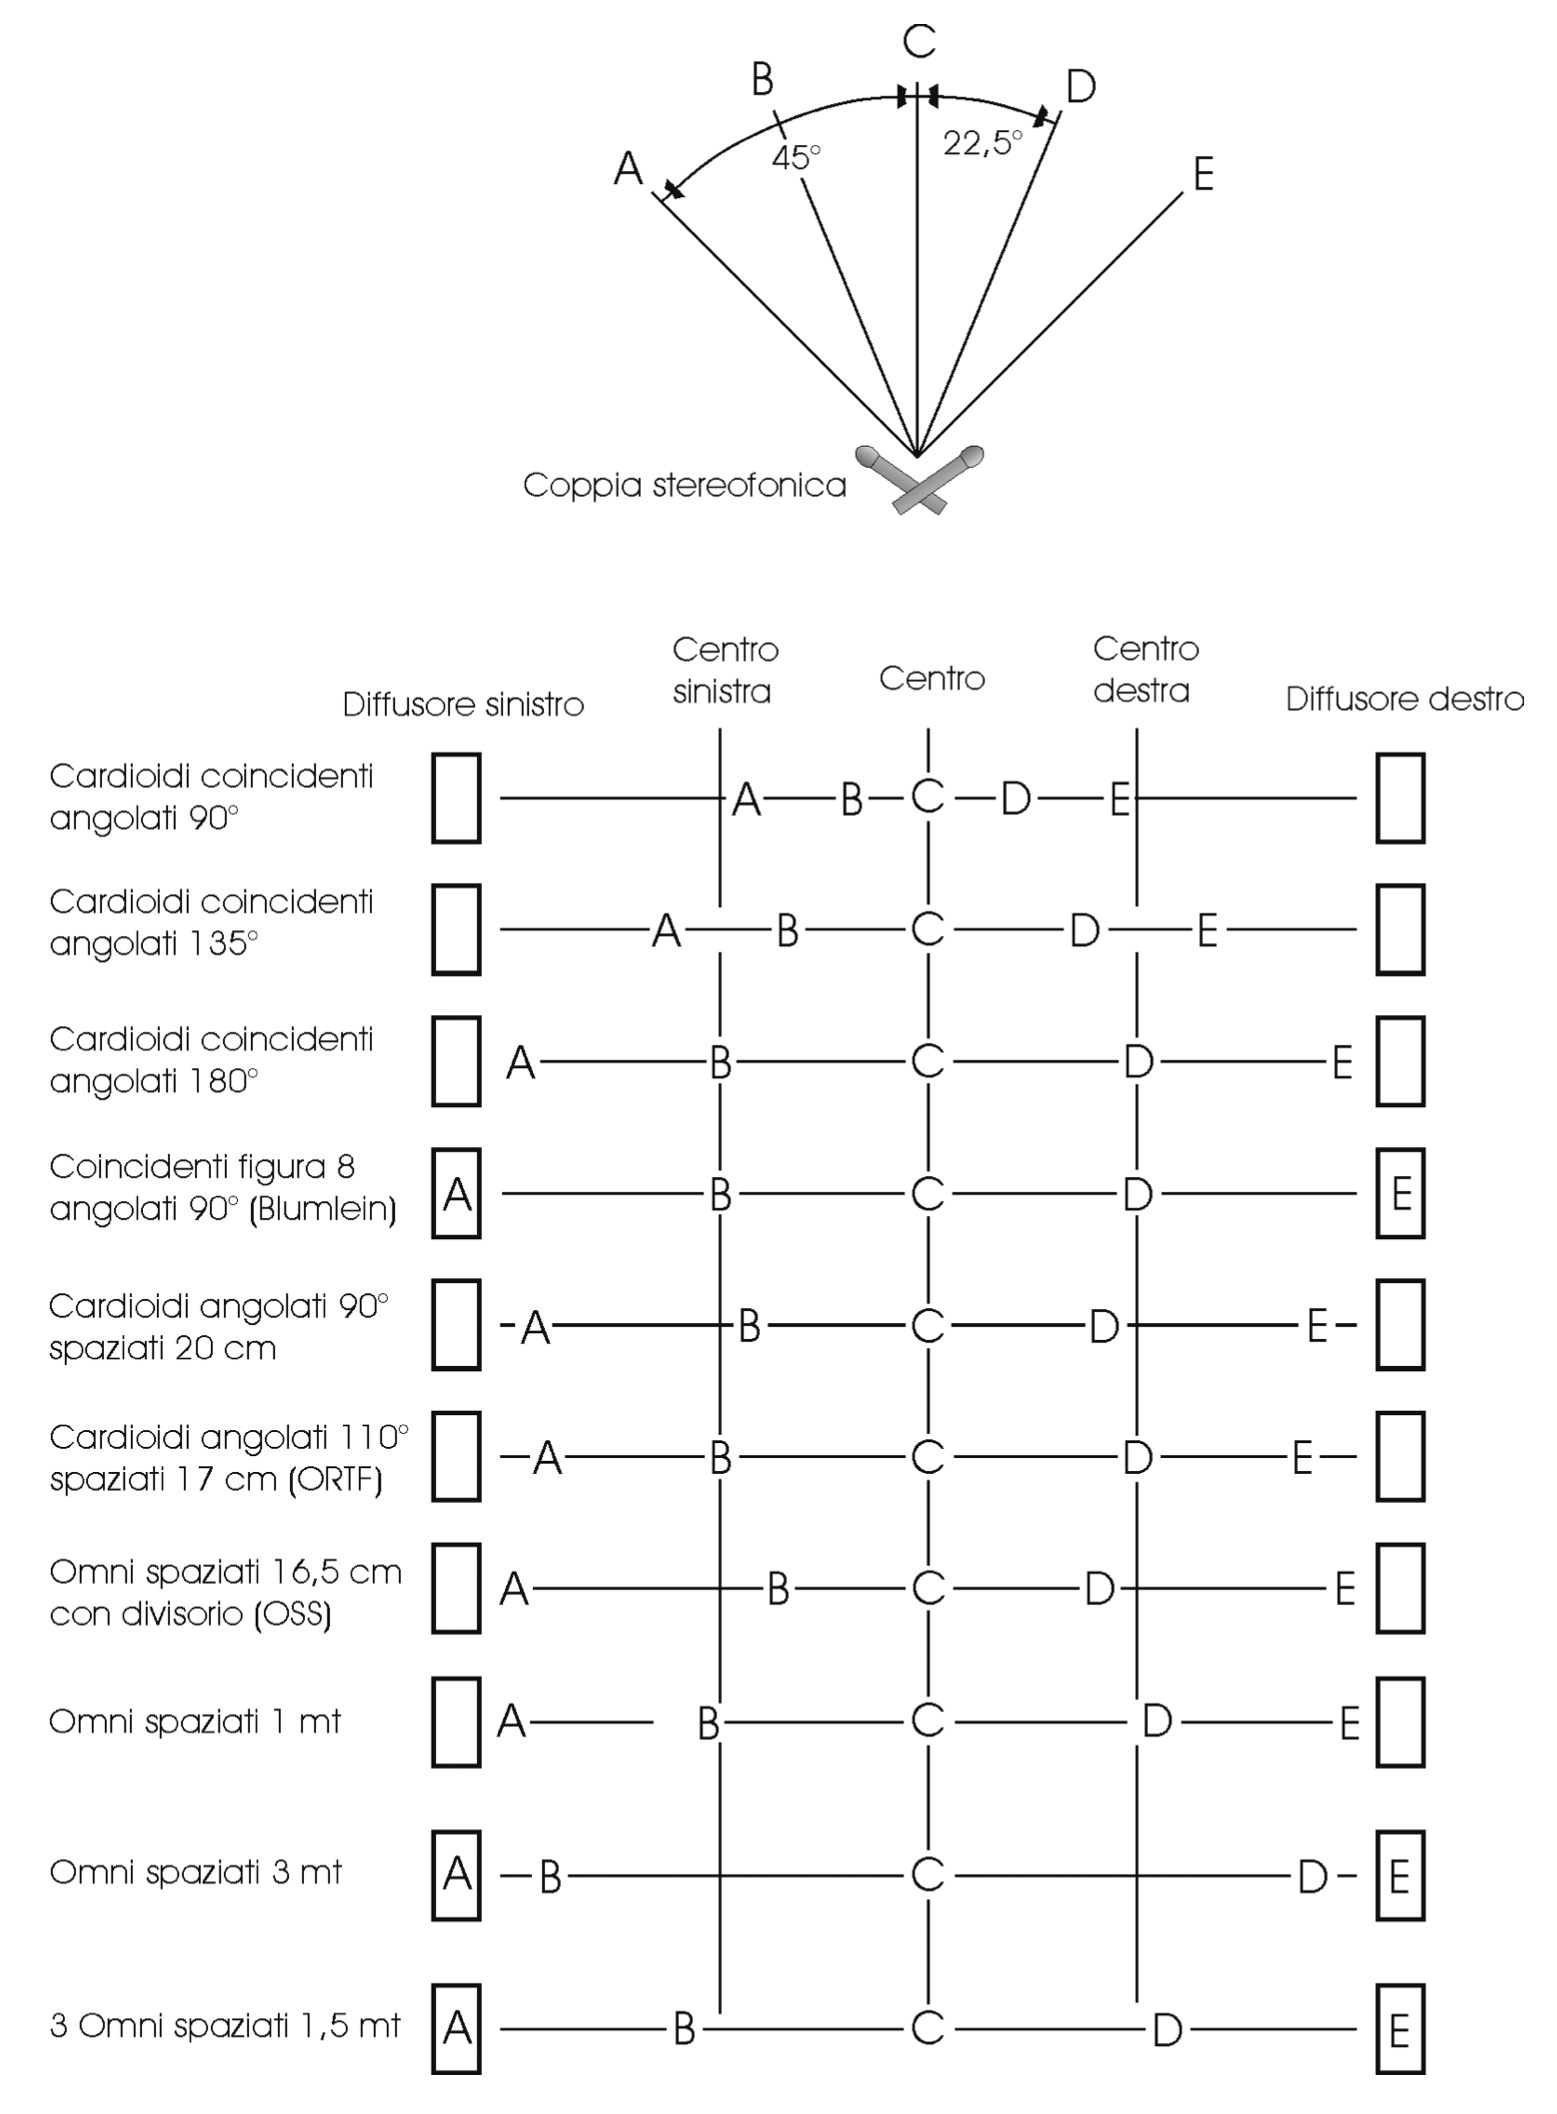
\includegraphics[width=0.99\columnwidth]{CAPITOLI/0300/IMG/localizzazione}
\caption[]{Ripresa di un fronte sonoro e localizzazione}
\label{fig:localizzazione}
\end{figure}

\subsection{Localizzazione}

La localizzazione è la capacità della ripresa di riprodurre una posizione degli
strumenti nello spazio orizzontale (da sinistra a destra) che si avvicini il più
possibile a quella originaria. Nella fig. \ref{fig:localizzazione} vediamo nella
parte superiore una coppia che riprende un fronte sonoro ipotetico di $90°$, e
in questo fronte sono evidenziati, oltre agli estremi (A e E), alcuni punti
intermedi (centro-sinistra B, centro C e centro-destra D). Nella parte inferiore
a differenti tecniche di ripresa, corrispondono differenti risultati di
percezione della localizzazione attraverso il riascolto con un sistema
stereofonico di diffusori: alcuni di questi si avvicinano in modo soddisfacente
alla riproduzione della posizione originaria, altri (ad es. la coppia coincidente
angolata di 90°) denotano una riproduzione ristretta, tendente a centrare i
suoni, altri (ad es. la coppia omni spaziata di 3 mt.) presentano, all’opposto,
una separazione eccessiva tra i canali ed un conseguente “buco” nel centro
d’ascolto.

\subsection{La definizione timbrica}

La definizione timbrica è dovuta in gran parte alla capacità di riprodurre la
gamma di frequenze originaria senza coloriture e senza perdite. Dando per
scontato l’utilizzo di microfoni professionali in cui l’accuratezza della
risposta in frequenza sia di livello adeguato, bisogna notare che il risultato
relativo a questo parametro dipende da diversi fattori: dalla caratteristica
polare del microfono stesso, dall’angolazione tra questo e la fonte sonora, e
dalla possibile influenza delle riflessioni dovute all’ambiente che possono, per
effetti di cancellazione di fase, alterare la risposta in frequenza del microfono
producendo colorazioni e buchi nella linearità della stessa.

\subsection{La profondità}

La profondità della ripresa non è altro se non la possibilità di distinguere,
all’interno del gruppo orchestrale, differenti piani sonori, come è nella realtà,
per cui gli archi devono risultare in un piano più ravvicinato rispetto ai legni,
collocati immediatamente alle spalle dei primi, e questi devono essere a loro
volta collocati davanti agli ottoni e alle percussioni. Naturalmente eventuali
solisti avranno la precedenza nei confronti della massa orchestrale, a meno che,
come nel caso delle riprese di opere liriche, si desideri mantenere il rapporto
scenico, con le voci più lontane rispetto all’orchestra. In mancanza della
definizione di questa dimensione, il problema può essere quello di un appiattimento
dell’orchestra su un piano orizzontale, con il risultato di una ripresa, magari
buona dal punto di vista degli altri parametri, ma poco interessante e coinvolgente.

\subsection{La spaziosità}

La spaziosità della ripresa consiste nella capacità di riproduzione dell’ambiente
in cui si effettua la ripresa, quindi una registrazione che voglia tener conto
di questo parametro conterrà una certa dose del riverbero ambientale presente
nella sala. Naturalmente, la misura del riverbero ambientale dovrà essere dosata,
oltre che dall’esperienza e dal gusto, dall’attenzione che deve essere posta nell
salvaguardia della definizione timbrica dello strumento. Anche qui, il risultato
dipenderà da diversi fattori: l’acustica della sala innanzitutto, e poi la scelta
della configurazione, nonché il posizionamento della coppia stessa. Un
posizionamento molto vicino allo strumento (o al gruppo orchestrale) darà un
rapporto suono diretto/suono riverberato più favorevole al suono diretto, rispetto
ad un posizionamento della coppia ad una certa distanza.

\subsection{Tipologie di coppie stereofoniche}

Entrando più in dettaglio sulle tipologie di configurazione, e partendo dal
presupposto di avere a disposizione due microfoni della stessa marca e dello stesso
modello e con caratteristiche simili (risposta in frequenza, curva polare, ecc.),
possiamo dividere le coppie in tre categorie:

\begin{compactitem}
\item coppie coincidenti
\item coppie quasi-coincidenti
\item coppie spaziate
\end{compactitem}

\subsection{Coincidenti}

Le coppie coincidenti, comunemente note come XY, consistono in due microfoni i
cui diaframmi di ripresa siano esattamente sovrapposti, in una vista ortogonale
dall’alto, una volta posti di fronte alla sorgente sonora. Una caratteristica
comune a tutte le coppie coincidenti è che offrono in assoluto la migliore
compatibilità mono, vale a dire che nel momento in cui si vadano a sommare i du
canali si hanno i minori fenomeni di cancellazione dovuti alle differenze di fase
dei due segnali.

\subsubsection{Blumlein}

Il primo esempio è dato dalla coppia coincidente figura-8 angolata di $90°$,
cioè la cosiddetta configurazione Blumlein, (a cui ci si riferisce come
inventore della stereofonia e di alcune tecniche di ripresa stereofonica). Come
si può vedere nella fig. 3, mentre il microfono corrispondente al canal
sinistro prende la parte sinistra dell’orchestra, per effetto della configurazione
a 8 prende anche l’ambiente retrostante destro, e inversamente farà l’altro canale.
Concettualmente, questa configurazione può essere pensata anche per quello che
ciascuno dei microfoni non prende (il sinistro non prende nulla del lato destro
dell’orchestra, coincidente col punto di annullamento massimo, e ugualmente
l’altro canale). Questa configurazione rimane una delle più precise come
equilibrio tra tutti i parametri sopra descritti.

Nella configurazione Blumlein è importante che il “fronte sonoro” sia contenuto
nell’apertura a 90° della coppia, per evitare l’influenza degli spostamenti di
fase dovuti al suono catturato dai microfoni nelle rispettive zone retrostanti.

\subsubsection{XY}

Usando due cardioidi in coppia coincidente, è possibile variare la loro
angolatura, così avremo una coppia angolata a $180°$, che darà una buona
localizzazione, a scapito di una scarsa definizione nella zona centrale,
dovuta al fenomeno per cui i suoni fuori-asse si attenuano nelle componenti più
acute, ed è una configurazione da tenere presente nel caso il fronte sonoro
sia limitato in ampiezza e si desideri avere una grande apertura sul
riverbero ambientale.

Angolando i microfoni a $135°$, avremo un miglioramento
della definizione, perché le curve polari, riducendo l’angolatura, tendono
sommare le risposte. Questa coppia ha una minore apertura stereo, è può essere
utilizzata quando si voglia raggiungere questo risultato.

Riducendo ancora l’angolatura, abbiamo la coppia angolata a $90°$ che, come
evidenziato nella tabella di fig. \ref{fig:localizzazione}, è la configurazione
che presenta la più ridotta apertura stereo, tendendo a concentrare i suoni
verso il centro. Può essere desiderabile quando il fronte sonoro è molto ampio
e si sia obbligati a riprenderlo molto da vicino.

\clearpage

\begin{figure*}[t]
    \centering
    \begin{subfigure}[t]{0.99\textwidth}
        \centering
        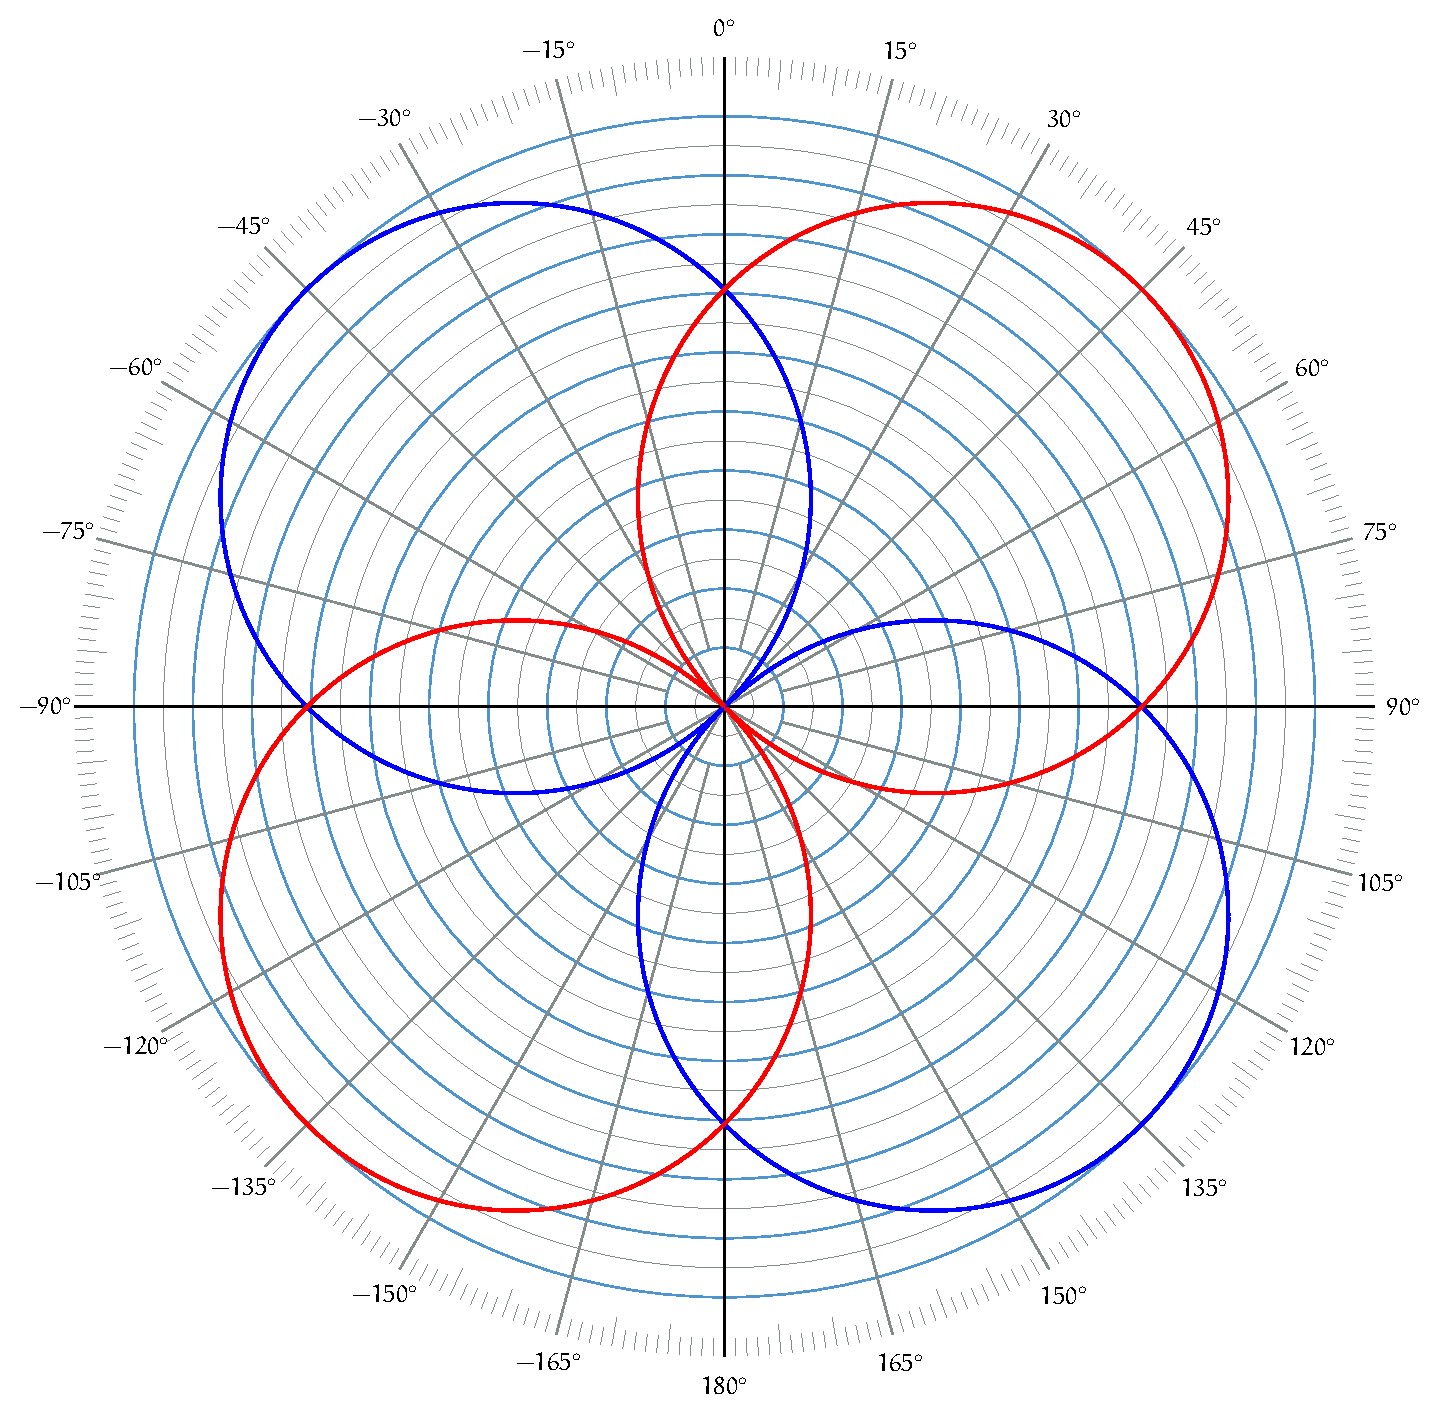
\includegraphics[width=11cm]{microphone-polar-patterns/blumlein}
        \caption[]{BLUMLEIN. Coppia stereofonica coincidente di figura-8 angolati tra loro di $90°$.}% \\ Eq: $1(x)$}
        \label{pol:blumleinsp}
    \end{subfigure}%
    \\
    \begin{subfigure}[t]{0.99\textwidth}
        \centering
        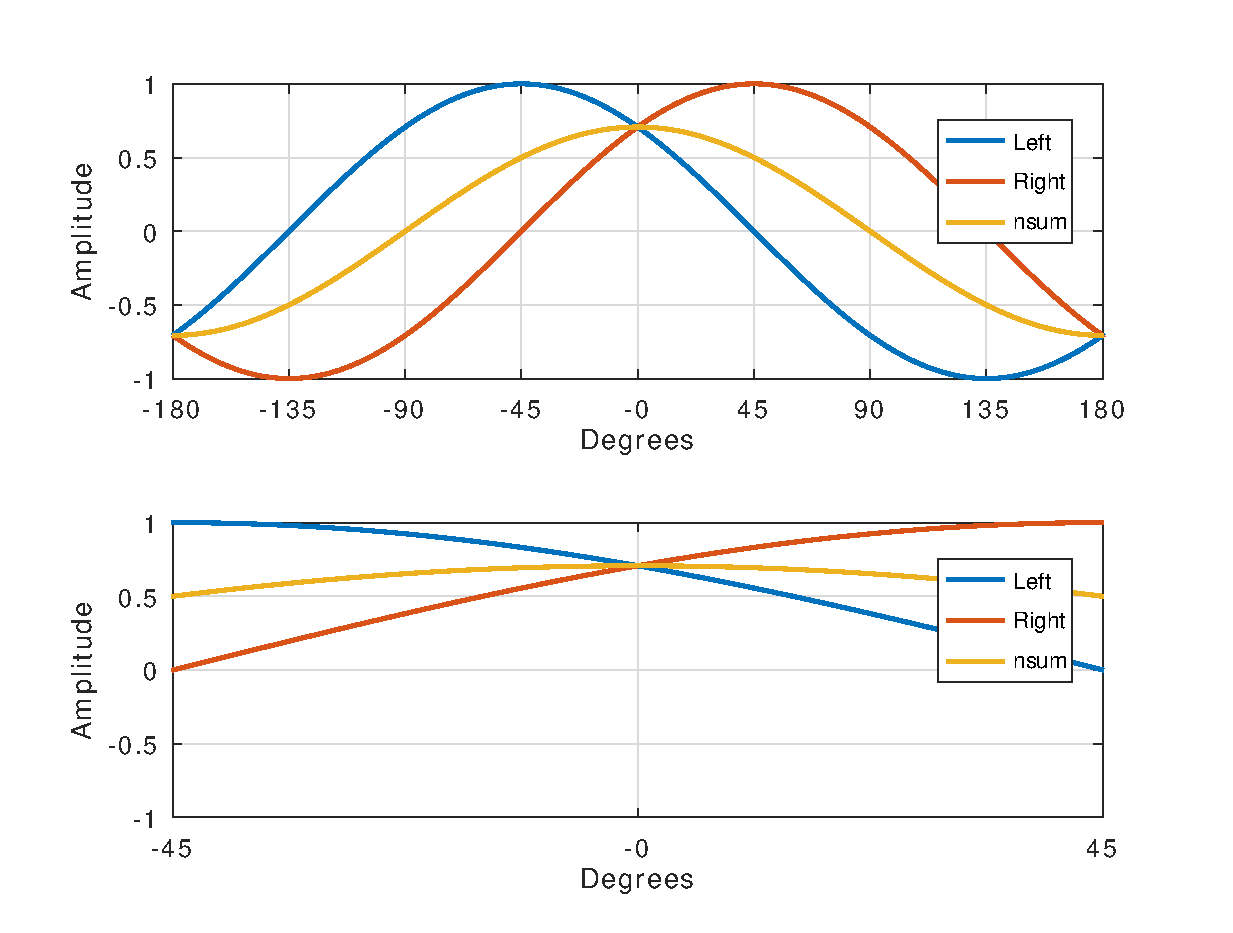
\includegraphics[width=12.5cm]{CAPITOLI/0300/IMG/blumleinsub}
        \caption[]{Variazioni angolari di ampiezza.}% \\ Eq: $0.75(x)+0.25(x\cos\theta)$}
        \label{plot:blumlein}
    \end{subfigure}
    \caption[]{BLUMLEIN}
    \label{sp:blumlein}
\end{figure*}

\clearpage

\begin{figure*}[t]
    \centering
    \begin{subfigure}[t]{0.99\textwidth}
        \centering
        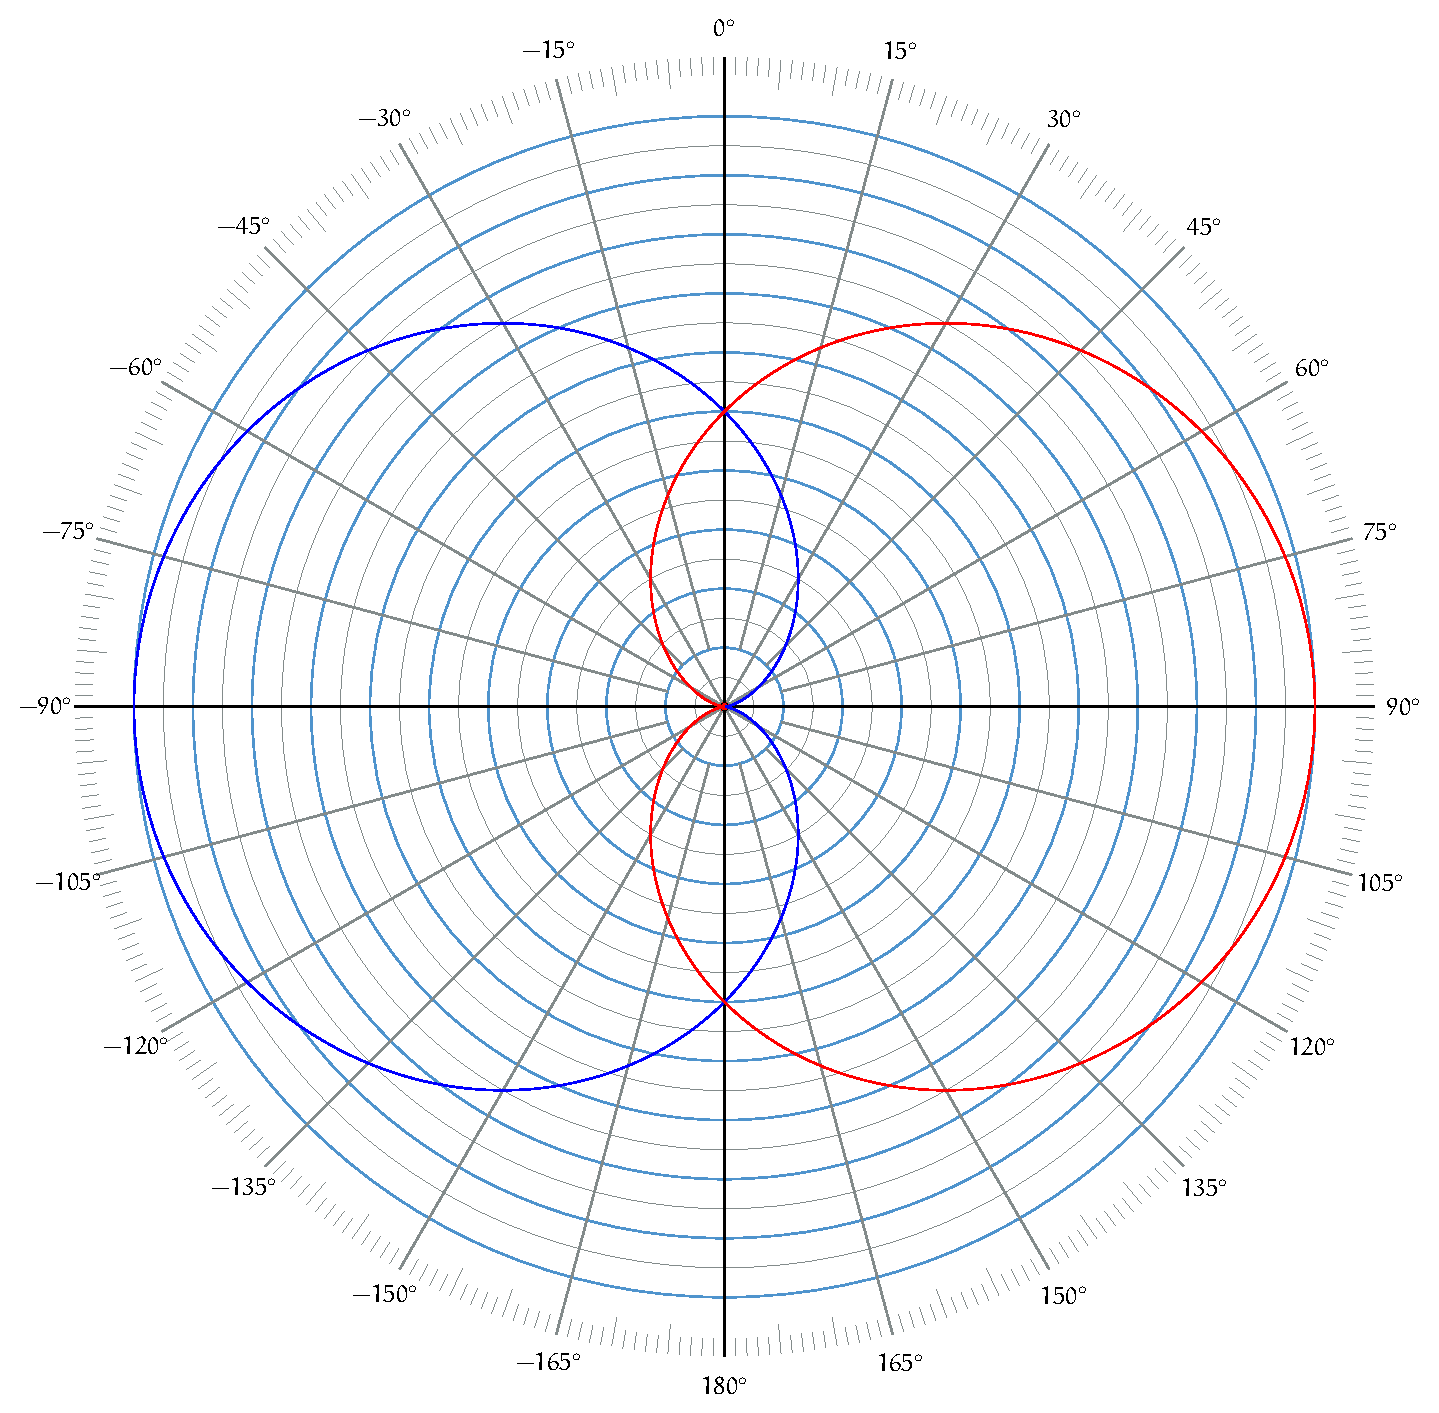
\includegraphics[width=11cm]{microphone-polar-patterns/xy180}
        \caption[]{XY90. Coppia stereofonica coincidente di cardioidi angolati tra loro di $180°$.}% \\ Eq: $1(x)$}
        \label{pol:xy120sp}
    \end{subfigure}%
    \\
    \begin{subfigure}[t]{0.99\textwidth}
        \centering
        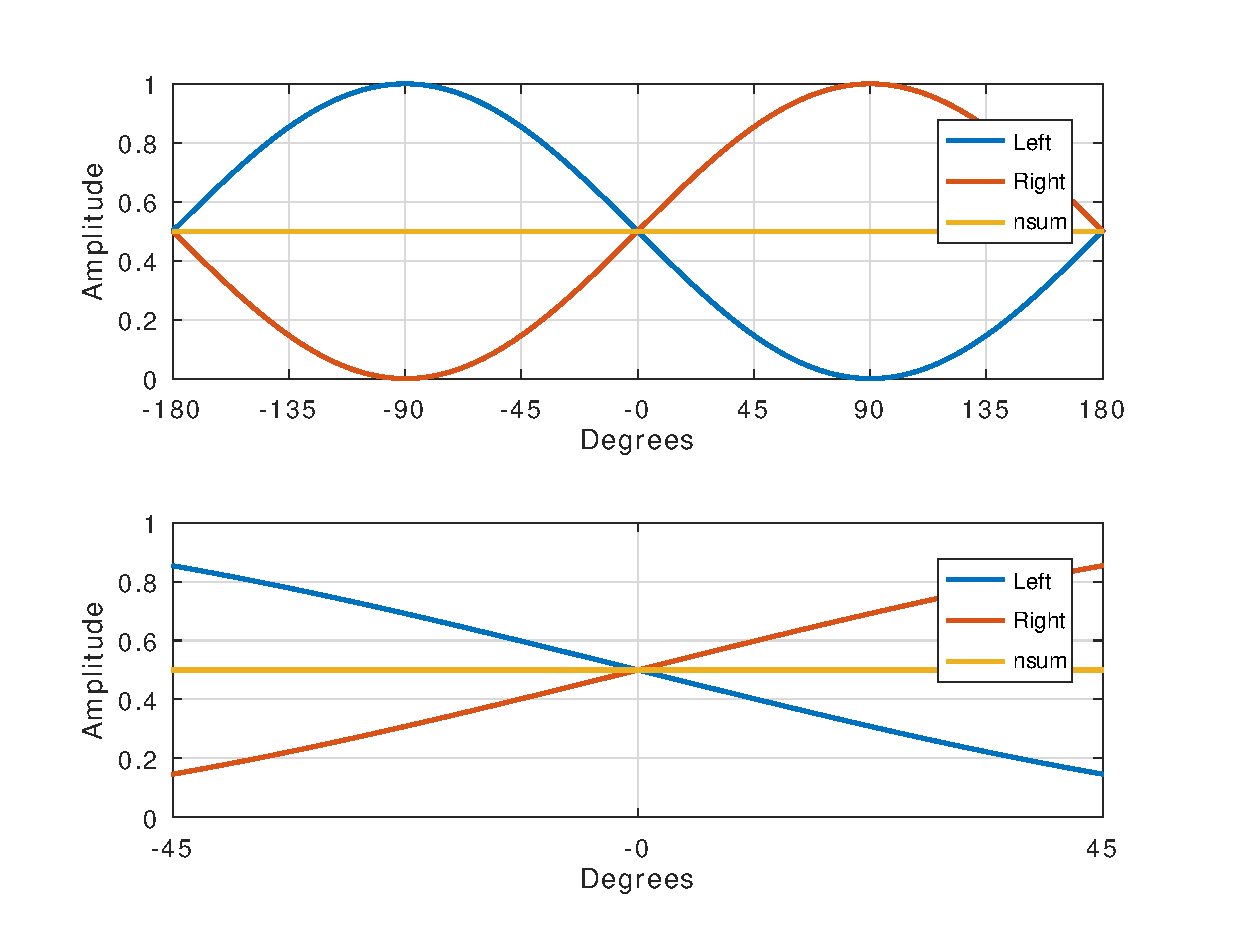
\includegraphics[width=12.5cm]{CAPITOLI/0300/IMG/xy180sub}
        \caption[]{Variazioni angolari di ampiezza.}% \\ Eq: $0.75(x)+0.25(x\cos\theta)$}
        \label{plot:xy180}
    \end{subfigure}
    \caption[]{XY180}
    \label{sp:xy180}
\end{figure*}

\clearpage

\begin{figure*}[t]
    \centering
    \begin{subfigure}[t]{0.99\textwidth}
        \centering
        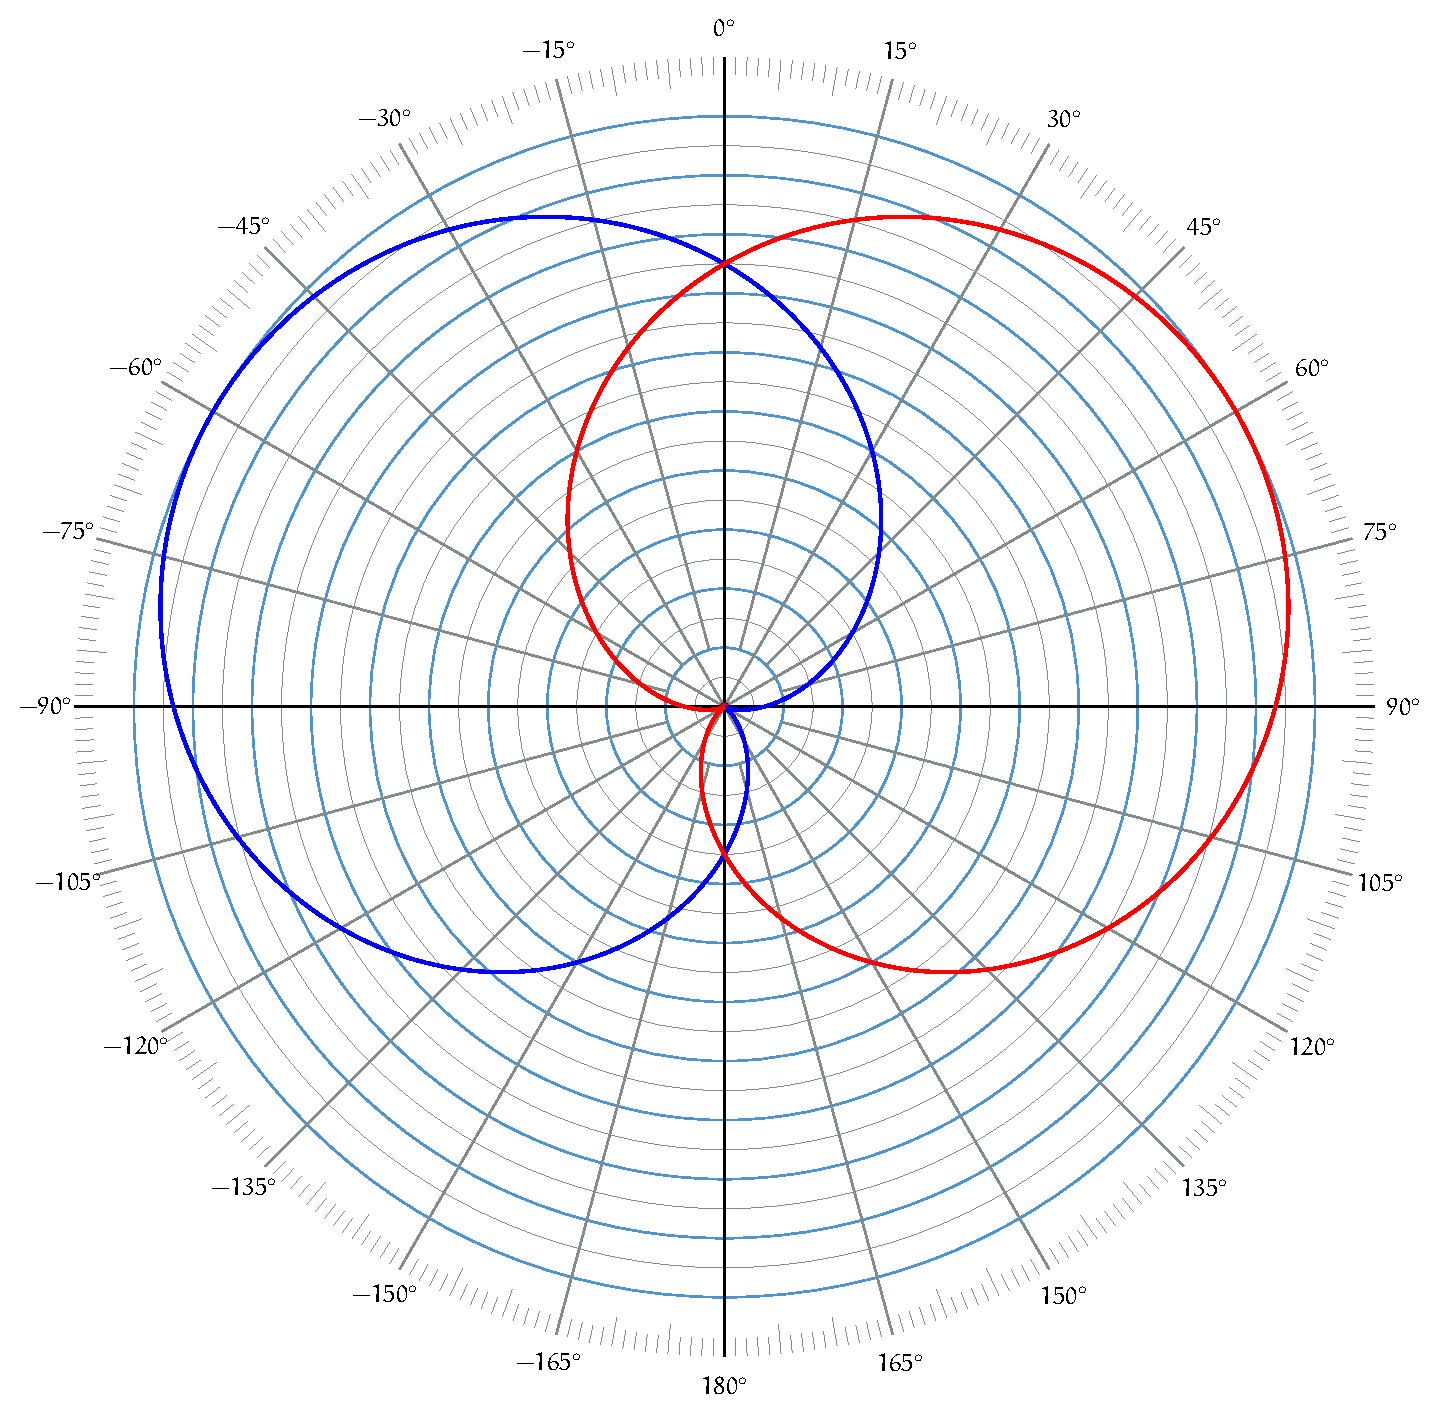
\includegraphics[width=11cm]{microphone-polar-patterns/xy120}
        \caption[]{XY90. Coppia stereofonica coincidente di cardioidi angolati tra loro di $120°$.}% \\ Eq: $1(x)$}
        \label{pol:xy120sp}
    \end{subfigure}%
    \\
    \begin{subfigure}[t]{0.99\textwidth}
        \centering
        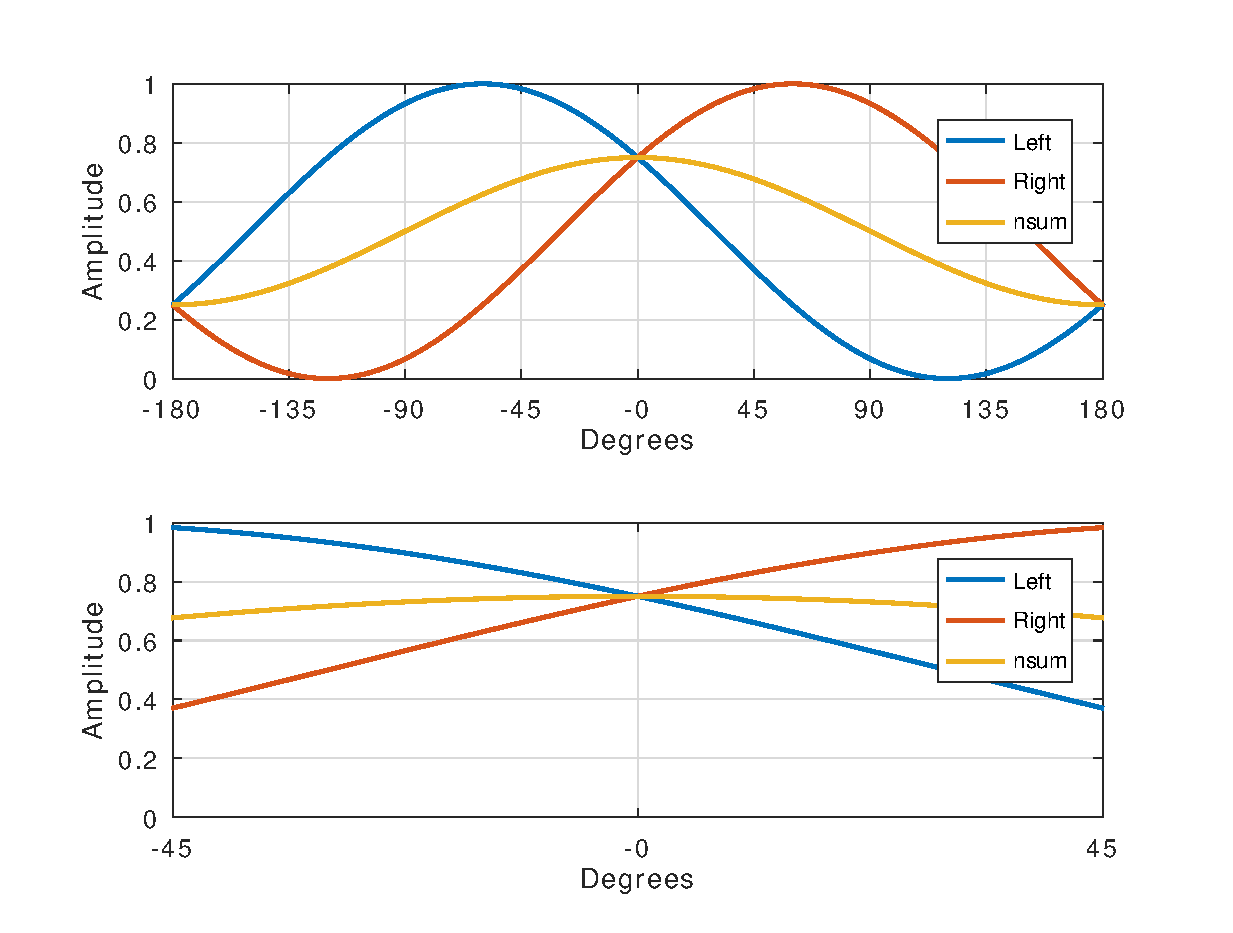
\includegraphics[width=12.5cm]{CAPITOLI/0300/IMG/xy120sub}
        \caption[]{Variazioni angolari di ampiezza.}% \\ Eq: $0.75(x)+0.25(x\cos\theta)$}
        \label{plot:xy120}
    \end{subfigure}
    \caption[]{XY120}
    \label{sp:xy120}
\end{figure*}

\clearpage

\begin{figure*}[t]
    \centering
    \begin{subfigure}[t]{0.99\textwidth}
        \centering
        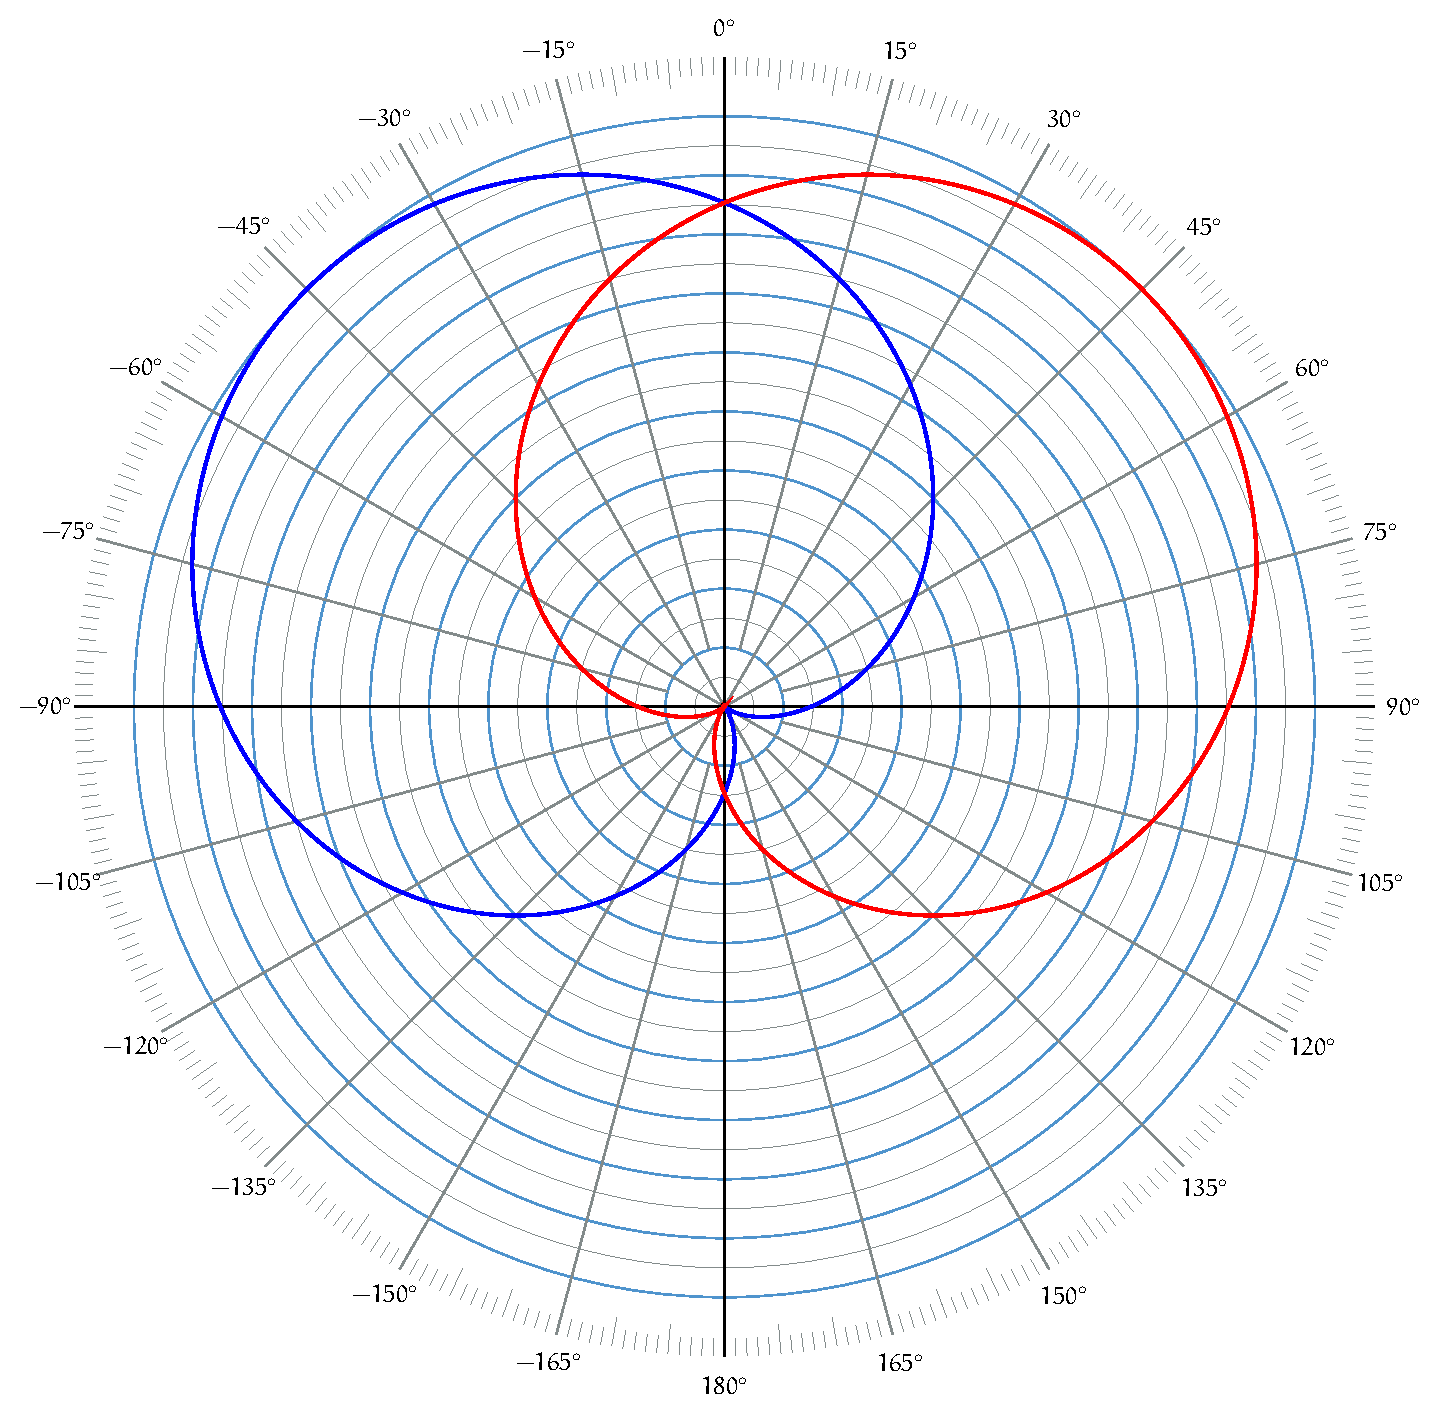
\includegraphics[width=11cm]{microphone-polar-patterns/xy90}
        \caption[]{XY90. Coppia stereofonica coincidente di cardioidi angolati tra loro di $90°$.}% \\ Eq: $1(x)$}
        \label{pol:xy90sp}
    \end{subfigure}%
    \\
    \begin{subfigure}[t]{0.99\textwidth}
        \centering
        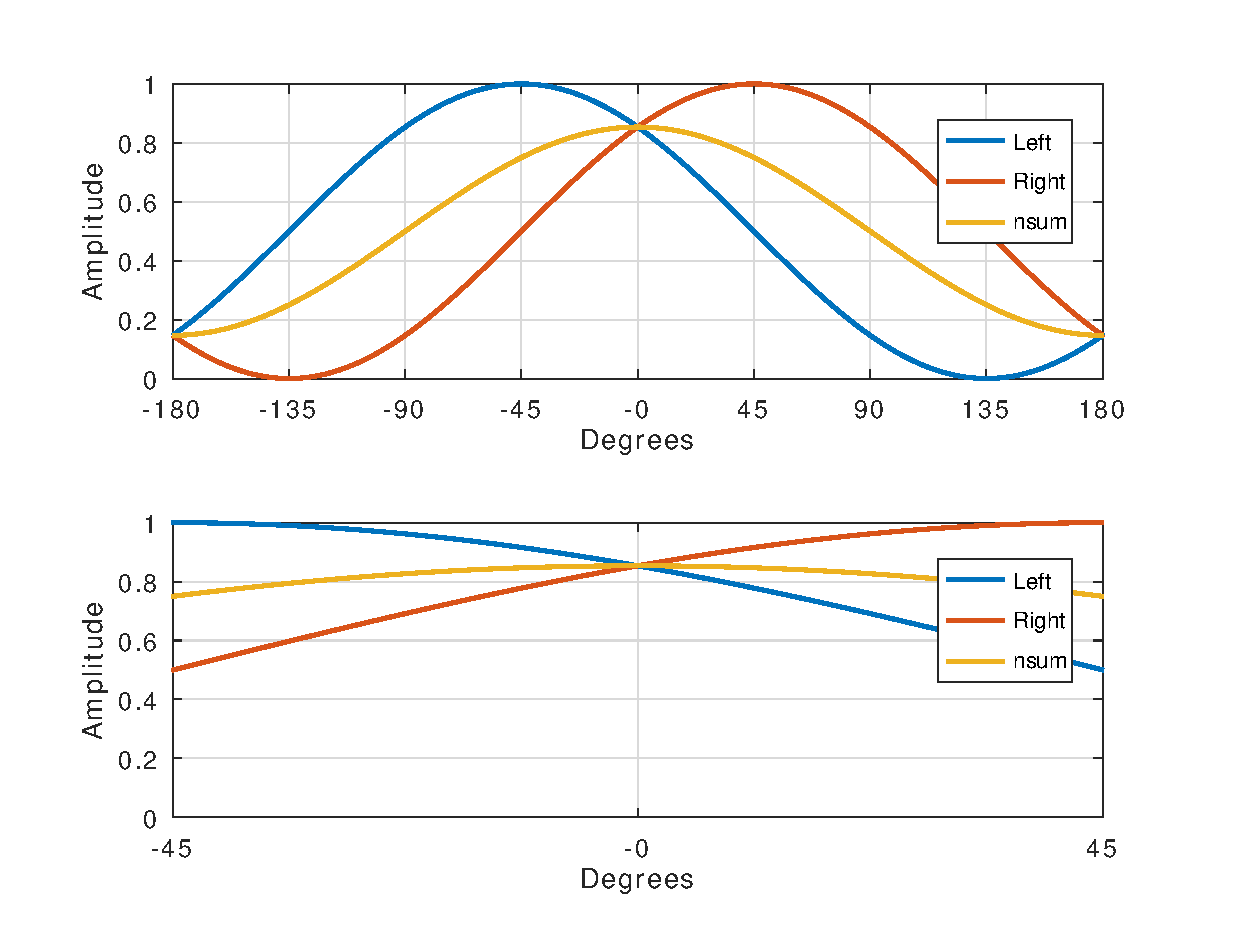
\includegraphics[width=12.5cm]{CAPITOLI/0300/IMG/xy90sub}
        \caption[]{Variazioni angolari di ampiezza.}% \\ Eq: $0.75(x)+0.25(x\cos\theta)$}
        \label{plot:xy90}
    \end{subfigure}
    \caption[]{XY90}
    \label{sp:xy90}
\end{figure*}

\clearpage

\subsection{Semi-coincidenti}

Le coppie quasi-coincidenti, rispetto a quelle esaminate fin qua, offrono una
maggiore ampiezza di immagine stereofonica ed una resa più ricca della riverberazione
ambientale. Per converso, diminuisce la compatibilità mono, in quanto allontanando
tra loro i diaframmi dei microfoni diminuisce la coerenza di fase, in special
modo alle alte frequenze.

Nella fig. \ref{pol:ortfsp} è illustrata una coppia angolata di $110°$ e spaziata
di $17cm$, la cosiddetta coppia ORTF, dal nome dell’allora ente radiotelevisivo
francese all’interno del quale è stata sviluppata. Può essere considerata i
assoluto come una delle migliori soluzioni per tutti i parametri sopra illustrati.

Un’altra coppia quasi-coincidente, la configurazione “DIN”, dove l’angolatura
è stata ridotta a 90° e la distanza tra le capsule portata a 20 cm. Come si può
constatare dalla tabella di fig. \ref{fig:localizzazione}, questo porta a
spostare verso il centro i suoni intermedi e ad allargare i suoni estremi.
Se la distanza viene portata a 30 cm la configurazione prende il nome di “NOS”.

\clearpage

\begin{figure*}[t]
    \centering
    \begin{subfigure}[t]{0.99\textwidth}
        \centering
        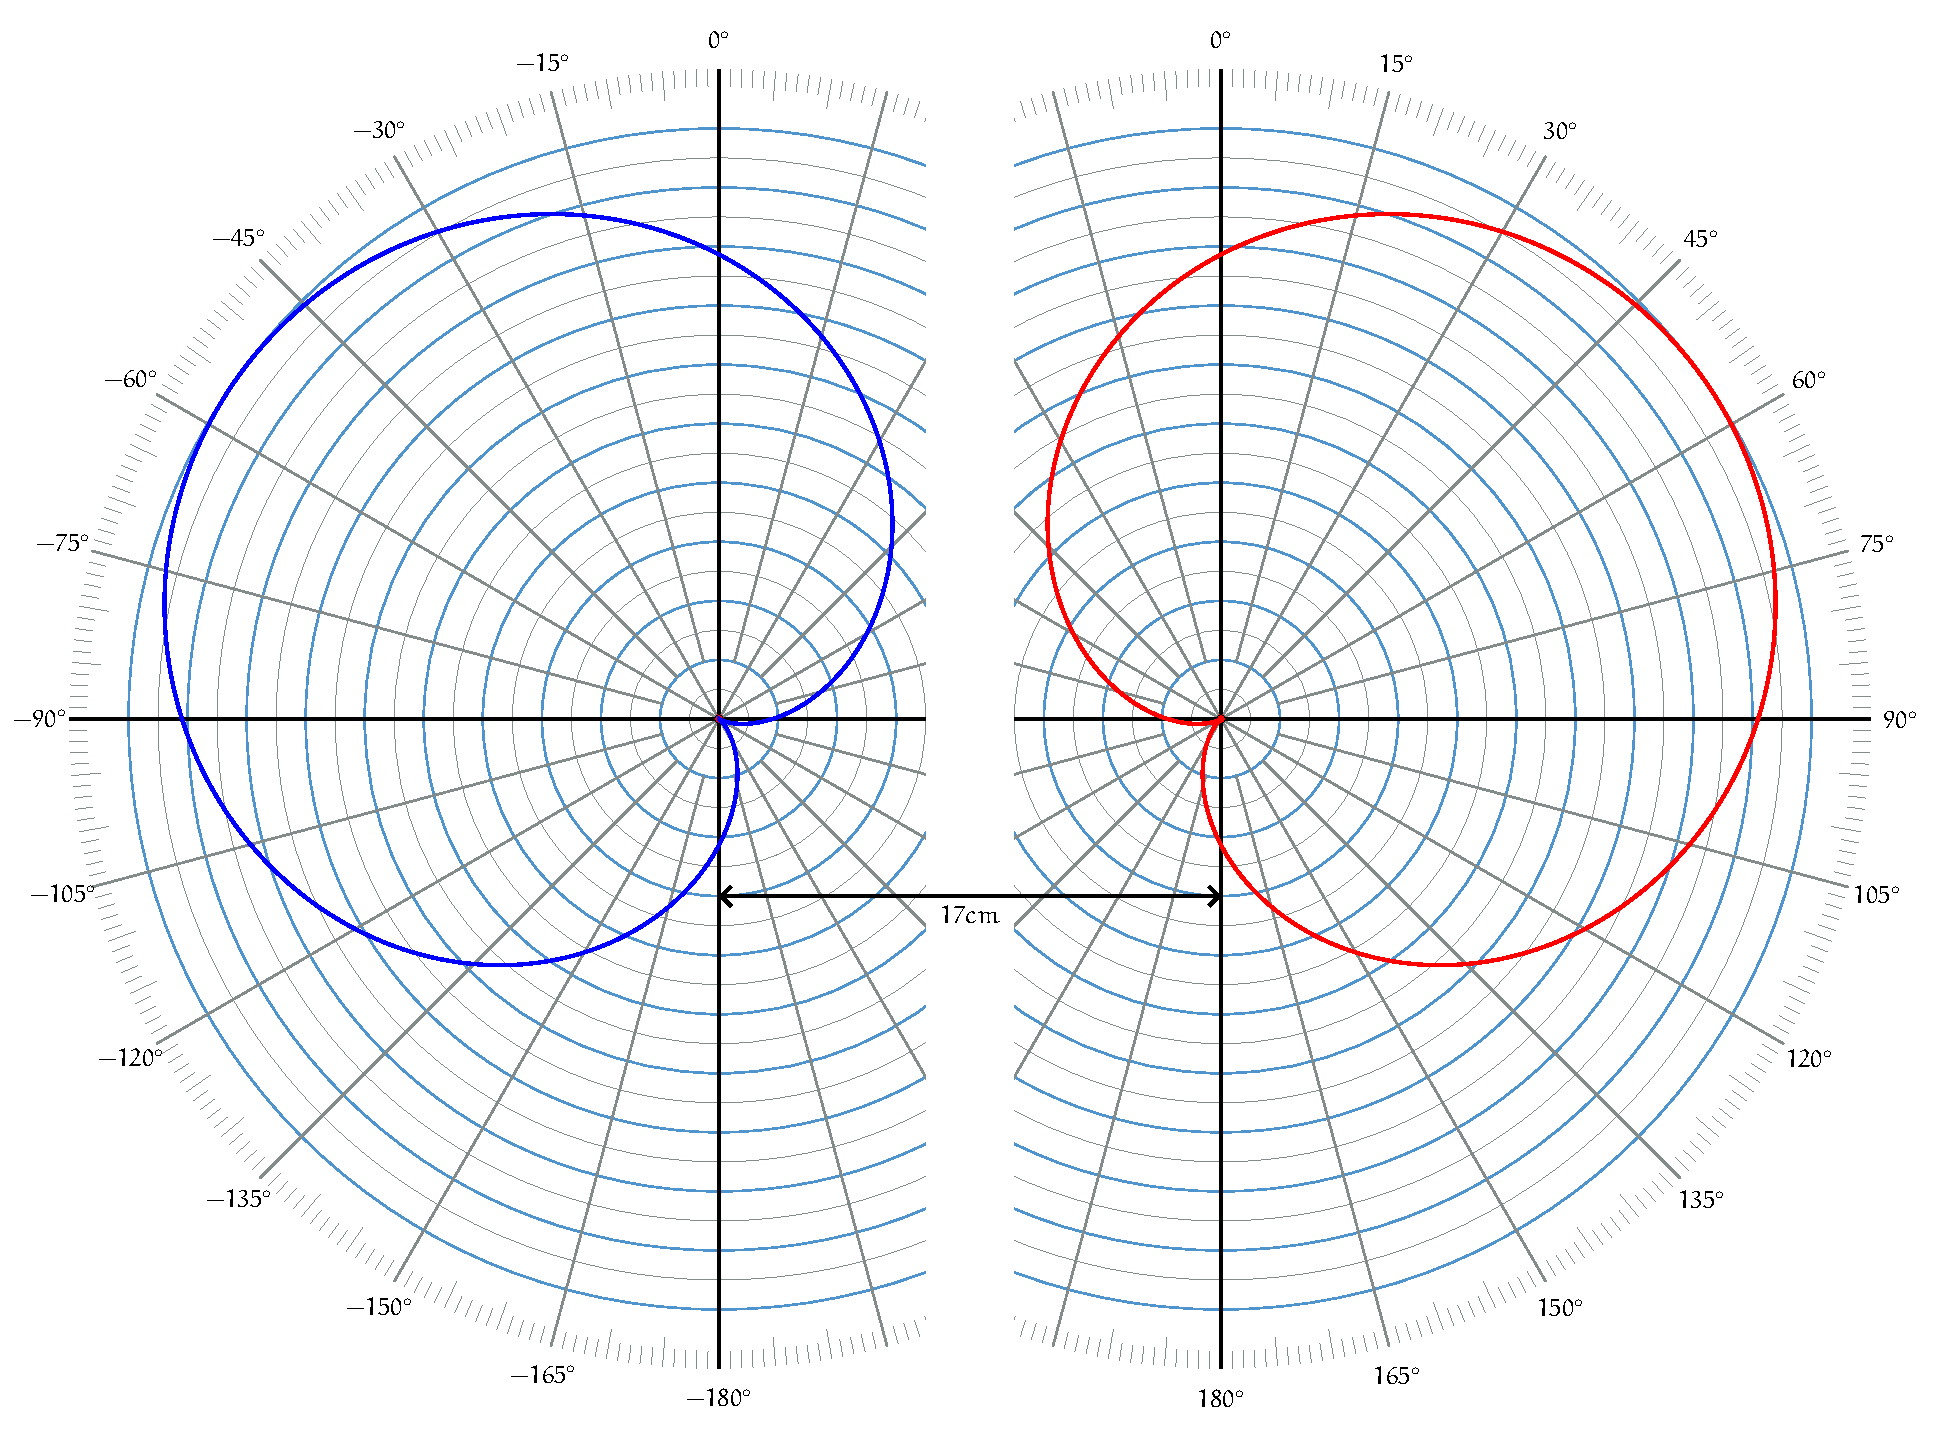
\includegraphics[width=11cm]{microphone-polar-patterns/ORTF}
        \caption[]{ORTF. Coppia stereofonica semi-coincidente di cardioidi angolati tra loro di $110°$ e distanti $17cm$.}% \\ Eq: $1(x)$}
        \label{pol:ortfsp}
    \end{subfigure}%
    \\
    \begin{subfigure}[t]{0.99\textwidth}
        \centering
        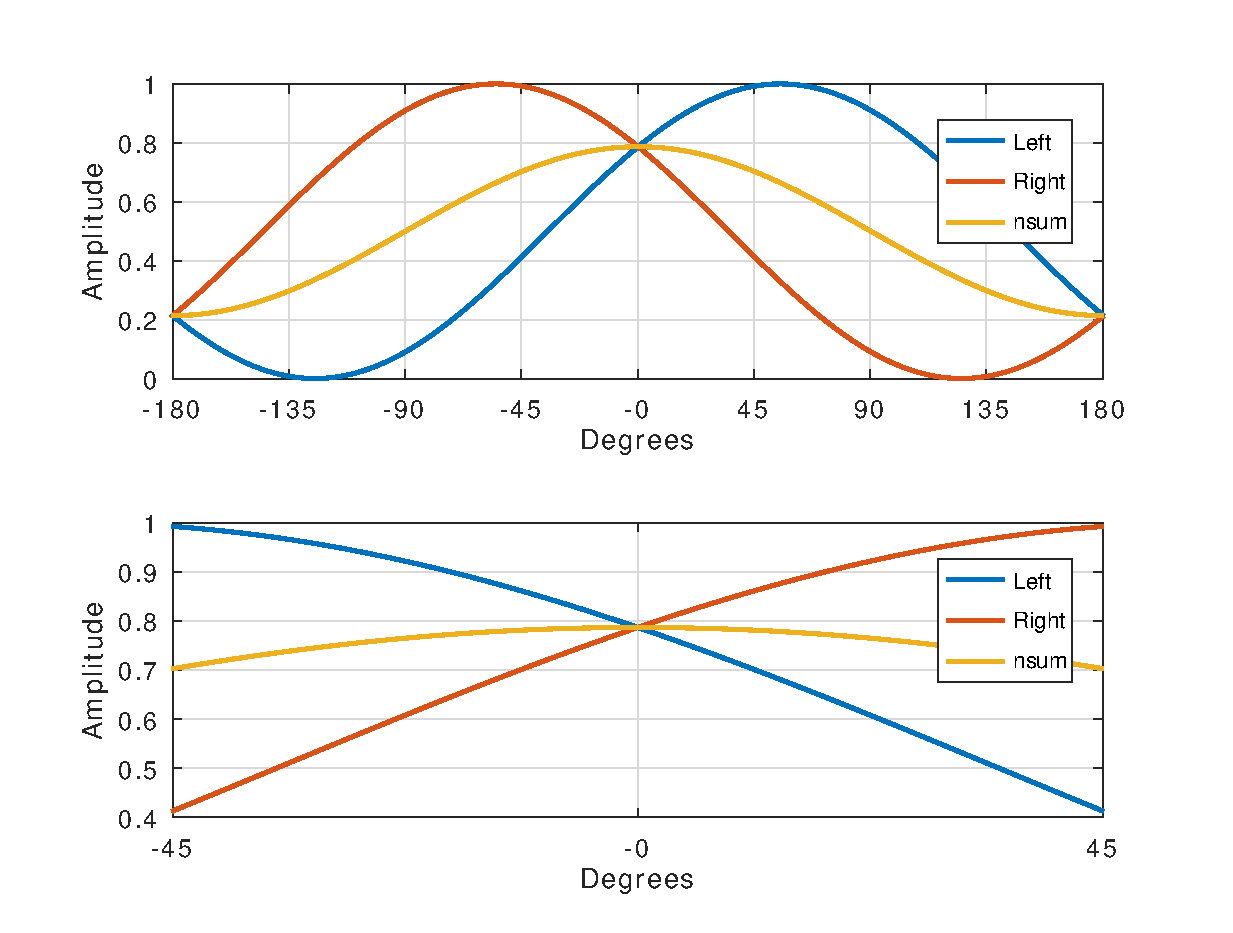
\includegraphics[width=12.5cm]{CAPITOLI/0300/IMG/ortfsub}
        \caption[]{Variazioni angolari di ampiezza.}% \\ Eq: $0.75(x)+0.25(x\cos\theta)$}
        \label{plot:ortf}
    \end{subfigure}
    \caption[]{ORTF}
    \label{sp:ortf}
\end{figure*}

\clearpage

\subsection{Le coppie spaziate}

Le coppie spaziate sono generalmente costituite da microfoni omnidirezionali
posizionati in parallelo tra di loro, rivolti verso la fonte sonora, e spaziati
di una certa distanza. Essendo entrambi i microfoni orientati nella stessa
direzione senza angolatura, la stereofonia è data dalla diversità di tempo
con cui il suono raggiunge i due microfoni, che si traduce anche in una
differenza di fase. E’ un tipo di ripresa molto adatto in ambienti dove il
riverbero ambientale è molto equilibrato, come ad es. un auditorium, in
quanto la capsula omnidirezionale riesce a restituire con ricchezza di dettaglio
anche gran parte del suono fuori asse. Altra caratteristica importante del
microfono omnidirezionale è la capacità di ripresa dei suoni gravi, superiore
a quella dei microfoni direttivi, per cui, nel caso di una registrazione
orchestrale, potrà rendere in maniera migliore suoni che si estendono molto
nella gamma bassa, come i contrabbassi, la grancassa, ecc. Va detto che tra
tutte le configurazioni è quella con la minor compatibilità mono, a causa delle
differenze di fase sopra descritte, per cui ove fosse impiegata in ripresa che
potrebbero avere un utilizzo in mono (ad es. riprese televisive), va usata con
prudenza e va controllato l’ascolto in mono per essere sicuri che non siano
avvertibili cancellazioni di fase.

%Nella fig. 10 la spaziatura è stata portata a 3 metri, e nella tabella di fig. 2 si può notare la differenza di questa ripresa rispetto alla precedente: gli strumenti tendono ad ammucchiarsi o tutti a sinistra o tutti a destra, lasciando un buco al centro.

%Nella fig. 11 nella configurazione precedente vediamo inserito un microfono centrale, che sul mixer sarà assegnato a entrambi i canali (left-right), con la funzione di ricreare il centro mancante. Questa configurazione, in realtà, non è più una coppia microfonica, essendo i microfoni tre, ma è generalmente considerata una variante delle configurazioni precedenti. In tale configurazione si usano indifferentemente sia microfoni cardioidi che omnidirezionali, e una grande cura deve essere posta nel posizionamento in vista di possibili effetti di “comb-filter” tra i tre microfoni.

Un ulteriore variante dei tre omnidirezionali è il cosiddetto “albero Decca”
(Decca tree), sviluppato dall’omonima casa discografica, dove il microfono
centrale è stato collocato in una posizione molto avanzata, in modo da dare
alla ripresa un centro assolutamente stabile, in conseguenza anche delle
differenze di tempo d’arrivo del suono. Il microfono preferito per questa
configurazione, quello con il quale questa configurazione è nata, è il
Neumann M50, ossia un microfono omnidirezionale a pressione dotato di una marcata
esaltazione delle frequenze alte in asse.

Un interessante configurazione è rappresentata dal sistema OSS (Jecklin disk),
in cui due microfoni omnidirezionali, spaziati di $16.5cm$, sono separati da un
divisorio rigido ricoperto di materiale fonoassorbente. Un tale sistema è vicino
alla simulazione di una testa umana, e può essere utile in riprese destinate
all’ascolto in cuffia (registrazioni binaurali).

Un’importante configurazione è la cosiddetta MS (mid-side), che consiste in un
microfono direzionale (cardioide o ipercardioide) sovrapposto ad un microfono
figura-8 disposto in modo da avere il punto di annullamento massimo in direzione
frontale. In tal modo, il microfono direttivo conterrà l’informazione relativa
al suono centrale (mid), mentre l’altro conterrà l’informazione relativa al
suono laterale (side).

%Il microfono mid entra in un canale e viene inviato, tramite il potenziometro panpot, ad entrambi i canali di uscita, mentre il microfono side viene fatto entrare su due canali, uno dei quali avrà il commutatore di fase invertito. Questi due canali vengono assegnati uno all’uscita sinistra e l’altro all’uscita destra, e potranno essere dosati e controllati tramite i relativi potenziometri del livello (fader). Il vantaggio di questa configurazione risiede proprio nella possibilità di separare l’informazione centrale da quella laterale, e di avere l’opportunità di controllare il bilanciamento di queste due informazioni.

%Un’ultima coppia stereofonica da segnalare è quella nota come “Testa artificiale” (Dummy Head, fig. 16), che consiste in una coppia di microfoni, generalmente omnidirezionali, installati all’interno di una struttura riproducente la conformazione di una testa umana, e posizionati in corrispondenza delle orecchie. Tale configurazione, tendente a simulare nel modo più accurato possibile la percezione umana, produce un tipo di registrazioni note come “registrazioni binaurali”, di cui tratteremo in seguito.

\subsection{Dummy Head}
